\section{Analysis}
%
\begin{figure}%
  \def\frac{0.24}
  % Ours with and without step loss
  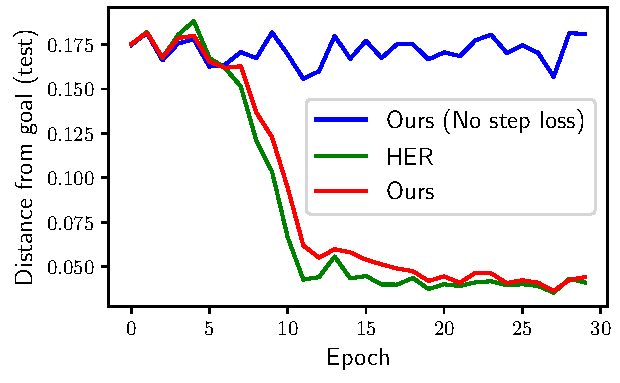
\includegraphics[width=\frac\columnwidth]{media/res/ablate-ddpg-with-without-step-loss/FetchPush-6efc1de-ddpgepoch-test/ag_g_dist.pdf}%
  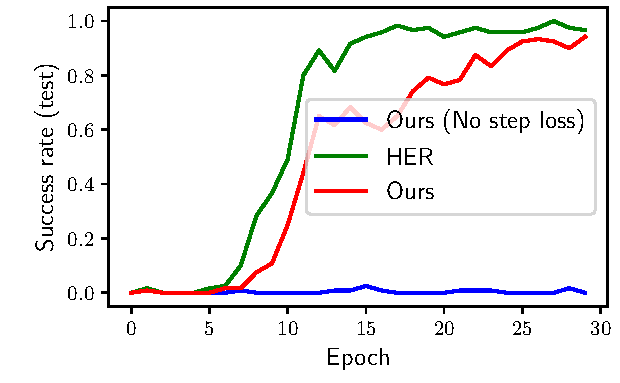
\includegraphics[width=\frac\columnwidth]{media/res/ablate-ddpg-with-without-step-loss/FetchPush-6efc1de-ddpgepoch-test/success_rate.pdf}%
  % Ours with and without goal rewards
  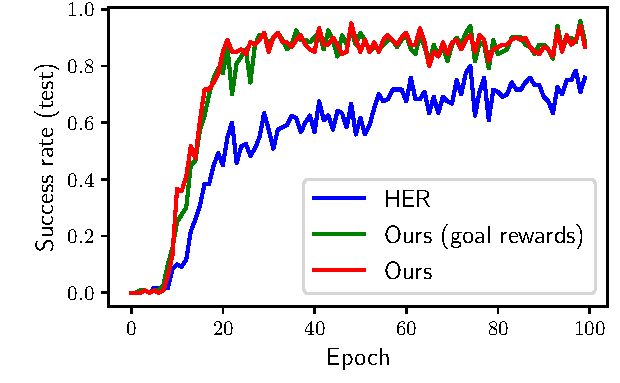
\includegraphics[width=\frac\columnwidth]{media/res/ablate-ours-with-goal-reward/FetchPickAndPlace-dqstepoch-test/success_rate.pdf}%
  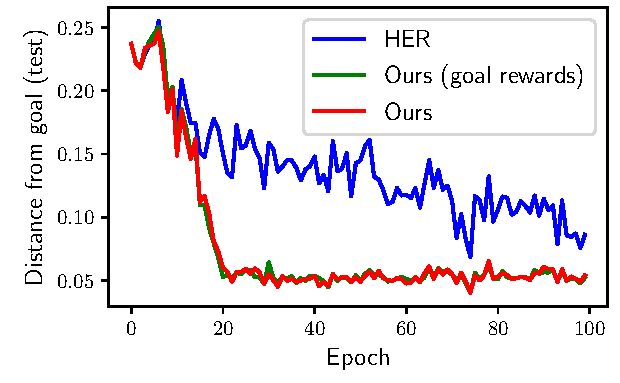
\includegraphics[width=\frac\columnwidth]{media/res/ablate-ours-with-goal-reward/FetchPickAndPlace-dqstepoch-test/ag_g_dist.pdf}%
  \label{fig:with-and-without-step-loss}%
  \caption{
    Effects of adding the goal-reward or removing the step-loss to our method.
    The left two plots on Fetch Push task show that the step loss is critical to the working of our
    method in the absence of goal rewards.
    The right two plots on Fetch Pick and Place task show that goal-rewards do not help much in raising the
    performance of our method. This shows that one-step loss captures the
    information that is equivalent to the providing the goal-rewards.}
\end{figure}%
% 

%
\begin{figure}%
  \def\frac{0.24}
  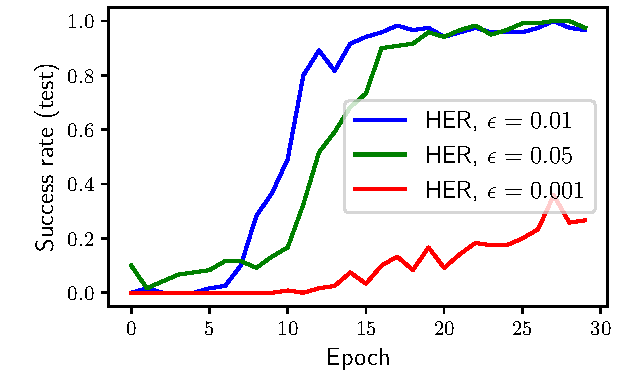
\includegraphics[width=\frac\columnwidth]{media/res/ablate-ddpg-dqst-low_tresh_chosen-low_thresh_alt-ddpg/0.05-be0910cepoch-test/success_rate.pdf}%
  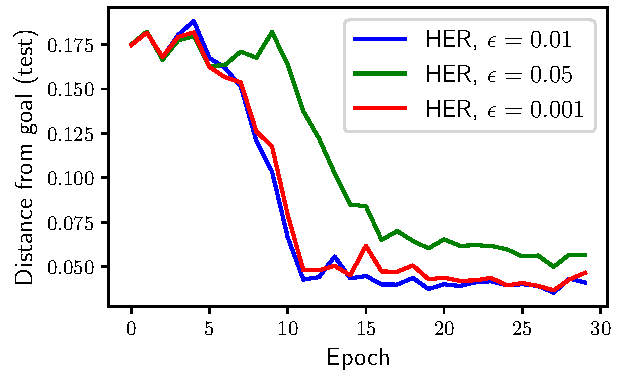
\includegraphics[width=\frac\columnwidth]{media/res/ablate-ddpg-dqst-low_tresh_chosen-low_thresh_alt-ddpg/0.05-be0910cepoch-test/ag_g_dist.pdf}%
  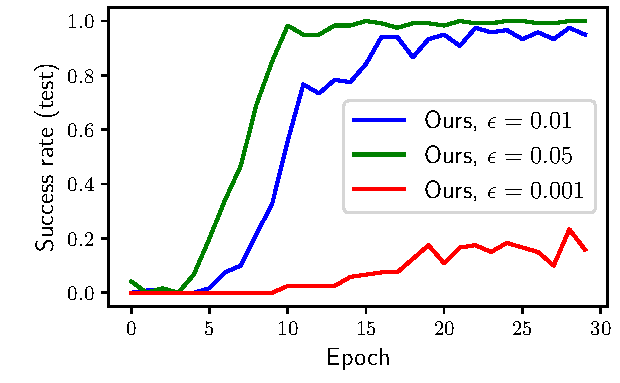
\includegraphics[width=\frac\columnwidth]{media/res/ablate-ddpg-dqst-low_tresh_chosen-low_thresh_alt-dqst/0.001-FetchPushPR-be467dfepoch-test/success_rate.pdf}%
  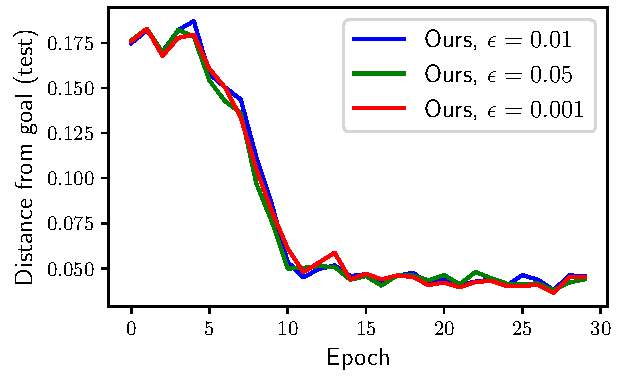
\includegraphics[width=\frac\columnwidth]{media/res/ablate-ddpg-dqst-low_tresh_chosen-low_thresh_alt-dqst/0.001-FetchPushPR-be467dfepoch-test/ag_g_dist.pdf}%
  \label{fig:with-different-distance-thresholds}%
  \caption{Effects of distance threshold on HER and our method on Fetch Push
task. Although the success rate decreases with decrease in distance threshold,
the distance to the goal is not affected by it. For HER the distance to the goal
reaches lower values with smaller distance thresholds.}%
\end{figure}%
% 

We perform three ask three additional questions about our algorithm:
(a) Do we really need the step loss?
(b) What happens when our algorithm has access to the goal reward?
(c) How critical is distance threshold to HER and our algorithm?
\paragraph{Do we really need the step loss?}
%
We run our algorithm with no goal reward and without the step loss on Fetch Push
task. This results in our algorithm failing to learn as shown in left two
columns of Figure~ref{fig:with-and-without-step-loss}.

\paragraph{Does our algorithm improves with access to the goal reward?}

We ran this experiment on Fetch Pick and Place task and found that goal-rewards
do not help much to our algorithm. The results are show in the right two columns
of Figure~\ref{fig:with-and-without-step-loss}. This indicates that one-step path reward
fully captures the information required for goal-conditioned tasks.

\paragraph{Effects of different distance thresholds}

In the absence of goal-rewards, our algorithm is not to able capture distance
threshold information that decides whether the agent has reached the goal or
not. On the other hand this information is available to HER. To understand the
sensitivity of our algorithm and HER on distance threshold, we vary the distance
threshold from 0.05 to 0.001 and show our results in
Figure~\ref{fig:with-different-distance-thresholds}.



